% Licensed to the Apache Software Foundation (ASF) under one or more
% contributor license agreements. See the NOTICE file distributed with
% this work for additional information regarding copyright ownership.
% The ASF licenses this file to You under the Apache License, Version 2.0
% (the ``License''); you may not use this file except in compliance with
% the License. You may obtain a copy of the License at
%
% http://www.apache.org/licenses/LICENSE-2.0
%
% Unless required by applicable law or agreed to in writing, software
% distributed under the License is distributed on an ``AS IS'' BASIS,
% WITHOUT WARRANTIES OR CONDITIONS OF ANY KIND, either express or implied.
% See the License for the specific language governing permissions and
% limitations under the License.


\subsubsection{Share Job Options}

You must complete the following tabs to configure a Share Job:

\bigimage{Share-edit-job-tab3}


\ifShareGuide
% Licensed to the Apache Software Foundation (ASF) under one or more
% contributor license agreements. See the NOTICE file distributed with
% this work for additional information regarding copyright ownership.
% The ASF licenses this file to You under the Apache License, Version 2.0
% (the ``License''); you may not use this file except in compliance with
% the License. You may obtain a copy of the License at
%
% http://www.apache.org/licenses/LICENSE-2.0
%
% Unless required by applicable law or agreed to in writing, software
% distributed under the License is distributed on an ``AS IS'' BASIS,
% WITHOUT WARRANTIES OR CONDITIONS OF ANY KIND, either express or implied.
% See the License for the specific language governing permissions and
% limitations under the License.

\begin{itemize}
\label{scheduling}

\item \textbf{Schedule type:} Whether you want to scan every document
once or dynamically recrawl content in your repository. 

When scanning every document once, the crawler marks all documents that
have been previously crawled in this job as potentially to be deleted,
adds all seed documents to its queue and marks them as pending, processes
pending documents, marking them completed as they are ingested, and then
deleted all of the documents that were not recrawled. A document might
not be recrawled because it no longer exists, or the job specification
might have been changed to no longer include the document.

When dynamically recrawling documents, the crawler does not start by
marking all documents as potentially deletable; instead, it begins with
all of the seed documents, and continues adding to its list, periodically
re-adding the initial seed documents. If a document is removed from the
source, it will expire in the expiration interval (see below).

\item \textbf{Expiration Interval (if continuous):} The length of the
interval (in minutes) that the appliance will retain a document
crawled by this job after the document no longer appears in the
repository. After this interval, the missing document will be removed
from the appliance's index and archive. Leave the expiration interval
blank to keep missing documents indexed in GTS.

\item \textbf{Recrawl interval:} If you are dynamically recrawling
documents, how long, in minutes, the crawler should wait before
crawling documents a second time.

\item \textbf{Reseed interval:} If you are dynamically recrawling
documents, how long, in minutes, the crawler should wait before
looking for new documents to crawl. \ifMeridioGuide This connector
identifies all documents for ingestion through seeding; if the reseed
interval is infinite, the job will not ingest documents placed in the
repository during run time. (The job automatically reseeds whenever it
is started.) The default interval of 60 minutes is an appropriate
reseed rate. \fi \ifFilenetGuide This connector identifies documents
for ingestion during seeding. If you change the document inclusion
criteria, reseeding is required to identify new documents. Similarly,
documents placed in the repository while the job is running will not
be identified until the crawl is reseeded.  (The job automatically
reseeds whenever it is started.) The default interval of 60 minutes is
an appropriate reseed rate. \fi

\item \textbf{Scheduled time:} Allows you to define a time you wish
the job to run using a series of selection boxes. The first box refers
to the day of the week you wish the job to run, with an option to have
the job run any day of the week. The second box allows you to select
the start hour, with an option to start the job at any hour. The third
box allows you to specify which minute after the hour that you wish
the job to start. The fourth box allows you to specify what months of
the year you wish the job to run, with an option for the job to run
any month. The last box allows you to specify the day of the month you
wish the job to start, including any day of month.


You can scroll through each of the five boxes in this setting using
the arrow keys on your keyboard or by using the scroll bar on the
right side of the box.  If you want to select more than one value,
hold down control as you scroll and click the values that you want to
select. This allows you to define multiple windows with the same
length, for example by selecting Monday, Wednesday, and Friday at the
same time.

\item \textbf{Maximum run time:} The longest you will allow the job to
run, in minutes. For example, if you want to start a job at 2 AM but
force it to stop at 8 AM so that users have access to the repository,
you should set this value to 360 minutes. If the job is not complete by the
end time, documents that have already been found will be indexed, and
the rest of the crawl will continue at the beginning of the next
schedule interval. 

When you have defined the scheduled time and assigned a maximum run
time, click on the ``Add Scheduled Time'' button. A new schedule box
will appear below the scheduled time, allowing you to create
additional scheduled run times.

Here is a sample schedule for a job that will run every
Monday from 2 am to 6 am:

\begin{changemargin}{-.3in}{0in} 
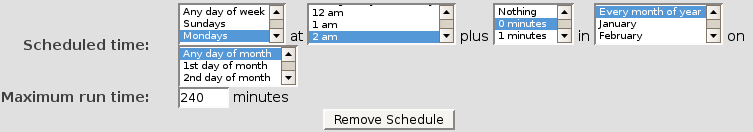
\includegraphics[width=300pt]{sample-schedule}
\end{changemargin}

If you do not have at least one scheduled time, the job will
only run when run manually (see page \pageref{ManageJobs}), and will
not automatically update the index on the appliance based on changes
to the repository.

You can remove a scheduled time by clicking the ``Remove Schedule''
button.

\end{itemize}

\fi

\ifCombinedConnectorGuide
This tab presents scheduling options. Here you can generate one or
more scheduled run times for the job. For a complete description of
the scheduling options, see the description starting on page
\pageref{scheduling}.
\fi


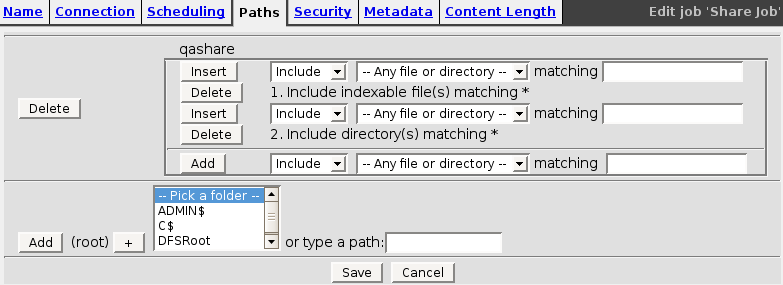
\includegraphics[width=300pt]{Share-edit-job-tab4}

\begin{itemize}

\item \textbf{Paths:} Here you can specify directory and file paths in
your network share from which you want your crawl to start. You can
specify one or more paths. If you do not specify any paths, the job
will not crawl any directories or documents. To generate each set of
paths, you must first build a directory path. You can build a
directory path by selecting individual directories. To start, you can
either select the base directory from the selection box or, if it does
not appear in the selection box, type its name in the empty text box,
then click the ``+'' button. A new selection box will appear with the
directories contained by that parent directory, along with a new text
box. Select or fill in a directory at that level and click the ``+''
button. Continue building your directory path in this fashion. When
it's complete, click ``Add''.

The directory path will appear along with a crawl customization
box. Using this customization box, you can use Windows file matching
expressions (or ``wildcard expressions'') to further specify directory and
file paths to crawl. Each path customization includes three parts. The
first selection is used to include or exclude items matched by a
wildcard expression. The second selection allows you to specify what
types of files and/or directories should be included with this
customization. The last part is a text box in which you can enter a
wildcard expression used to match files and/or directories. Complete
all three fields and click ``Add'' to insert the wildcard expression
instruction at the end of the list of instructions.

The list of wildcard expression instructions is evaluated from top to
bottom. Customization boxes appear in between list items, allowing the
insertion of instructions into the list. A wildcard expression
instruction can be deleted from the list by clicking the ``Delete''
button that appears next to it. By default, the list of instructions
includes two statements, \command{1.~Include file(s) matching *} and
\command{2.~Include directory(s) matching *}. Together these
instructions tell the job to crawl all contents contained by the
parent directory path.

Wildcard expressions use wildcard characters to match file and
directory names. The character \texttt{*} is used to match any zero or
more characters, while the character \texttt{?} matches any single
character. The brackets characters \texttt{[]} match any single
selection of characters that appears within the brackets. Simply
entering \texttt{*} as an expression matches everything. Some other
possiblities:

\begin{itemize}

\item \texttt{file??.txt}: A sequence of text files with a two digit
identifier.

\item \texttt{file*.txt}: A sequence of text files with a variable
length identifier.

\item \texttt{*.txt}: Any text file.

\item \texttt{*Data}: Any directory whose name ends with the word
``Data''.

\item \texttt{[abc]*}: Any file or directory whose name begins with
``a'', ``b'', or ``c''.

\item \texttt{*.[abc]*}: Any file whose extension begins with ``a'',
``b'', or ``c''.

\end{itemize}

You can continue to add more directory paths to your list using the
new selection box that appears below your completed directory
path. Each directory path can be customized with instructions as
described above. To remove a directory path from the list, click the
``Delete'' button next to it.

\end{itemize}

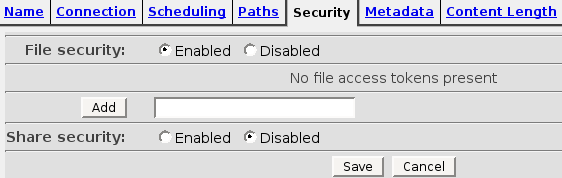
\includegraphics[width=300pt]{Share-edit-job-tab5}

\begin{itemize}

\item \textbf{File Security:}  Allows you to control whether or not file ACLs,
or access control lists, are passed to the appliance with the files.

\item \textbf{Access Tokens:} If you want to pass on your own Active
Directory ACLs instead of those of the network share you can enter
them here. You should enter one or more SIDs that you want to have
read permissions on the files crawled in this job. For more
information about AD ACLs and SIDs, please see the security sections
of the \documentref{MetaCarta Appliance Administrator's Guide}.

\note{If you have disabled security, these ACLs will not be passed to
the appliance.}

\item \textbf{Share Security:} In some cases, your network share's
security may include share security. You should enable or disable
share security to match your network share's security model.

\end{itemize}

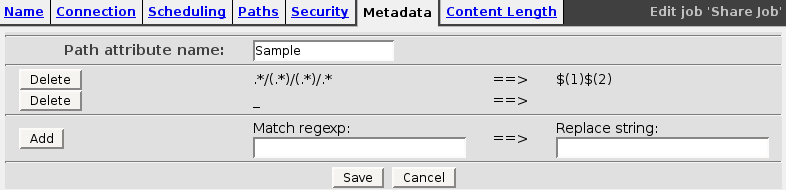
\includegraphics[width=300pt]{Share-edit-job-tab6}

\begin{itemize}

\item \textbf{Path Attribute name:} You can create a metadata field
to contain attributes from the file path. You can enter a name
for the metadata field here. It may be useful to have the metadata
field containing path attributes have the same name across jobs.
This metadata will not be geographically parsed or used to create the
index on the MetaCarta appliance; however, with MetaCarta Search APIs,
you can construct searches based specifically on this metadata. For more
information on the SOAP Search API, please see the \documentref{MetaCarta
SOAP Search API Guide}, and for more information on the JSON and KML
Search APIs, please see the \documentref{Web Services Search Guide}.

\item \textbf{Path-value mapping:}The regular expressions and
substitutions that you want to use to collect information from the
file path. You can construct one or more regular expressions. In the
example shown, there are two expressions. The first,
\verb+.*/(.*)/(.*)/.*+ to \verb+$(1) $(2)+, would change the directory
path ``Project/Folder\_1/Folder\_2/ Filename'' into ``Folder\_1
Folder\_2.'' The second, \_ to a space, would then be applied to turn
the metadata into ``Folder 1 Folder 2.'' It is important to allow more
than one transform so that you can, if necessary, extract text data
and then parse the extracted data. The end result of the last
transform will be ingested as the value of the metadata attribute
defined previously. \ifCombinedConnectorGuide If you are not familiar
with regular expressions, please see the note on page \pageref{regex}
for more information.\fi

\ifShareGuide 
\label{regex} 

\note{If you are not familiar with regular expressions, there
are a variety of tutorials available on the web, including
\url{http://gnosis.cx/publish/programming/regular_expressions.html}
and \url{http://}\linebreak \url{perldoc.perl.org/perlrequick.html}. If
you still have difficulty with these settings, please contact Customer
Support (see page \pageref{SupportContact}).} 

\fi

\end{itemize}

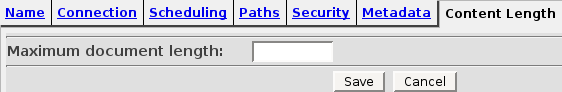
\includegraphics[width=300pt]{Share-edit-job-tab7}

\begin{itemize}

\item \textbf{Content Length:} The maximum file size, in bytes, that
you wish this job to crawl. Files larger than this size will be
skipped. The default maximum content length is unlimited.


After entering this information, you will be taken to the status page
for this job:

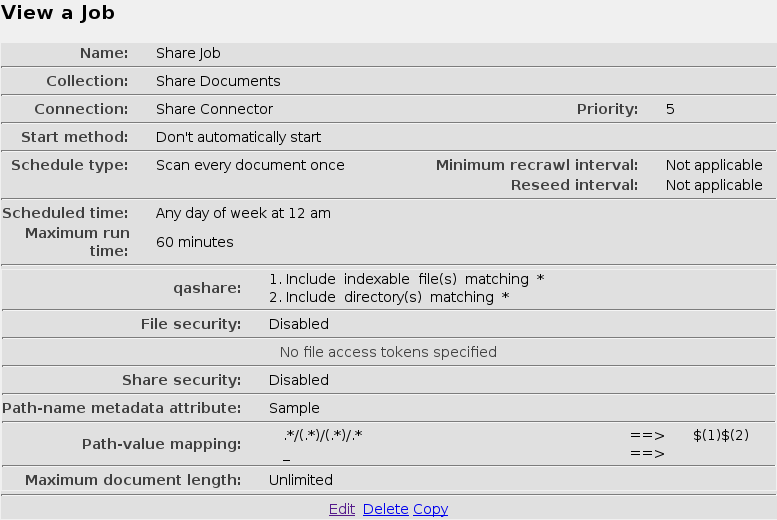
\includegraphics[width=300pt]{Share-view-job-status}


\end{itemize}

